\section{Requirements and Goal Definition}\label{sec:Requirements}
Before discussing and describing the concepts and findings in details for this study, it is important to define the goals. Without a definition and a description of goals, system development is more difficult to implement. Requirements Engineering comes to role at this stage. After the technology concepts have been explained on the basis of these requirements, the final concept is selected on the basis of various evaluation criteria, which are themselves ranked according to importance.

\subsection{Introduction to Requirements Engineering}
In this thesis, we deal with development of algorithms and software. Hence, it is essential to understand the methods which are industry standards for developing software. SDLC stands for Software Development Life Cycle. It is a process that defines the steps or phases that a software development project goes through from the initial planning stages to the final implementation and maintenance of the software.

The SDLC process is usually divided into several phases, which may vary depending on the specific method used, but commonly include:

\begin{itemize}
    \item Requirements gathering and analysis: This phase involves understanding the needs of the users and stakeholders, and identifying the functional and non-functional requirements of the software.
    \item Design: This phase involves creating a detailed design of the software, including the system architecture and user interface.
    \item Implementation or coding: This phase involves writing the code for the software based on the design.
    \item Testing: This phase involves testing the software to ensure that it meets the requirements and is free of bugs.
    \item Deployment: This phase involves installing the software on the target system and making it available for use.
\end{itemize}

The SDLC process helps to ensure that the software is developed in a structured and organized way, and that the final product meets the needs of the users and stakeholders. Different SDLC models such as Waterfall, Agile, V-Model, Spiral Model, etc can be used depending on the needs of the project and the organization.

V Model, Waterfall, and similar methods are all traditional SDLC models that are often used in requirement engineering. The V Model is a software development process that follows a linear and sequential approach, with each phase of the process flowing in a V-shape from the requirements phase to the testing phase. The model is based on the idea of "verification and validation", where the requirements are verified during the design phase, and the system is validated during the testing phase.These methods are commonly used to plan, design, and build a product. They are not part of Requirements Engineering but they rely on requirement engineering as the first phase. The Requirements Engineering phase is where the requirements are gathered, analyzed, and specified before the design and development of the product begins.

Of all the methods mentioned, below is a brief explanation of one of the most used SDLC model before discussing requirements engineering :
V-Modell is a German software development process model that is widely used in Germany and other German-speaking countries. It is a phased, linear, and sequential model that is often used in government and defense projects. The model is based on the idea of "verification and validation" where the requirements are verified during the design phase, and the system is validated during the testing phase.

The V-Modell is divided into four main phases:
\begin{itemize}
    \item Planning and Organization: This phase involves defining the project goals, outlining the project plan, and identifying the project team.
    \item Analysis and Concept: In this phase, the requirements are gathered, analyzed, and specified. This includes defining the system architecture, and creating a detailed project plan.
    \item Realization: This phase involves the design, development, and implementation of the system. This includes the coding, testing, and integration of the system.
    \item Deployment and Maintenance: This phase involves the deployment of the system, the training of users, and the maintenance of the system.
\end{itemize}

The V-Modell also includes several intermediate phases such as the "System Design" and "System Test" phases. These phases are focused on verifying and validating the requirements at different stages of the development process. The V-Modell also includes specific guidelines for documentation, quality assurance, and project management.

\begin{figure}[!h]
    	\centering
    	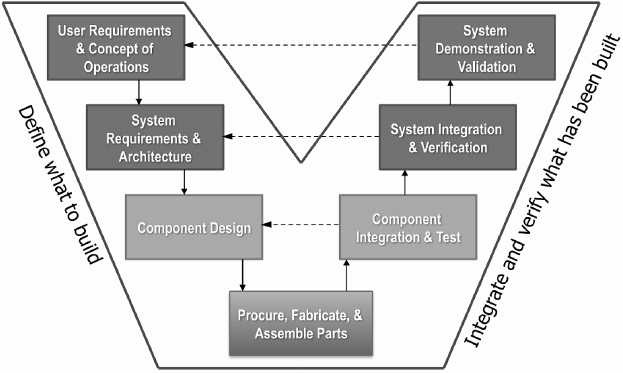
\includegraphics[width= 0.85\textwidth]{images/Typical-systems-engineering-V-model.png}
    	\caption [V-Modell]{V-Modell Diagram \protect\cite{vmodel}}  
    	\label{fig:V-Modell}
\end{figure}

One of the main advantages of the V-Modell is its focus on the verification and validation of requirements. This helps to ensure that the end product meets the needs of the customer, while also taking into account safety, performance, and other critical factors. However, the V-Modell can be inflexible and may not be suitable for rapidly changing environments where the requirements may evolve over time.
The first step of this approach is to make a list of requirements and define them. In the table given below, a list of requirements with their brief definition is provided. Additionally, the type of requirement is also mentioned. 


Every project will have certain requirements that are defined to be Must-Have (MH). It is imperative that these requirements are met in order to deem the project successfully completed. These requirements are called MVP or Minimum Viable Product. MVP is a concept that is often used in product development and management. It refers to the version of a product that has just enough features to be able to be released to a limited group of customers (often called "early adopters") and gather feedback. The idea is to validate the product's value proposition and gather feedback before investing more resources into development. MVPs are often used in the context of lean startup methodologies, which prioritize learning and validation over the pursuit of a perfect product. So MVP is a concept that can be used in product management but it is not a part of product management. Once the MVP has been created one would always want to have more features added to the tool/program for enhanced sophistication. Such features are part of the requirements which are defined as Nice-to-have (NTH) requirements. These requirements can include things like additional convenience features, aesthetics, or performance improvements. They are not essential for the core functionality of the product, but they can add value and make the product more attractive to customers.

\begin{table}[h]
    \centering
    \begin{tabular}{ |p{4cm}||p{4cm}||p{4cm}|}
     \hline
     \textbf{Requirements} & \textbf{Description} & \textbf{Type of Requirement} \\
     \hline
     Compression Factor & Achievable compression without loss of data  & MH\\
     \hline
     User Friendly & Ease of access for end-user & MH  \\
     \hline
     Data Evaluation Capability & Capability to evaluate and utilize compressed data for additional purposes & MH  \\
     \hline
     Troubleshooting Friendly & End-user must be able to troubleshoot algorithm/program errors with ease & MH  \\
     \hline
     Multi-format program & The compression should be applicable to as many file types as possible & NTH \\
     \hline
     Extensibility & Possibility to modify the algorithm/program for additional features in future & NTH \\
     \hline
     Data Re-usability & Encryption and Decryption of compressed data should be possible, if applicable & NTH\\
     \hline
     Data Evaluation  & Capability to utilize compressed data and perform data evaluation as desired & MTH \\
     \hline
    \end{tabular}
    \caption{List of Requirements}
    \label{tab:Requirements List}
\end{table}

\clearpage



